\chapter{Model-Free Deep Hedging of Variable Annuities}

\section{Introduction}

Reinforcement Learning (RL) is a branch of machine learning that focuses on training algorithms, known as agents, to make a sequence of decisions. 
The agent learns to achieve a goal in an uncertain, potentially complex environment by trial and error, using feedback from its own actions and experiences. 
Unlike supervised learning, where training data is labeled with the correct answers, in RL, an agent is provided with rewards or punishments as signals for its actions.

The core of RL revolves around the concept of the agent interacting with its environment over time, aiming to maximize the cumulative reward. 
This process involves observing the state of the environment, selecting and performing actions, and receiving rewards or penalties in response to those actions. 
The agent's objective is to learn a mapping from states to actions that maximizes this cumulative reward, which is often referred to as a policy. 
One of the fundamental frameworks for modeling RL problems is the Markov Decision Process (MDP). 
An MDP provides a mathematical formulation of the decision-making process, characterized by states, actions, rewards, and transition probabilities. Solving an MDP involves finding a policy that maximizes some function of the expected rewards, typically the expected cumulative reward over time.

Reinforcement learning algorithms can be broadly categorized into two types: model-based and model-free approaches. 
Model-based methods utilize a model of the environment to simulate the outcomes of actions, enabling planning and decision-making with fewer interactions with the environment. 
Conversely, model-free methods learn directly from interactions with the environment, without relying on a model, making them more straightforward but often less efficient in terms of sample usage.

A compelling application of RL is in the hedging of financial derivatives, a domain where the complexity and uncertainty of financial markets make traditional static models inadequate.
Financial derivatives are contracts whose value is derived from an underlying asset, and hedging is the practice of making investments to reduce the risk of adverse price movements.
RL's adaptability and learning capabilities offer a promising solution to dynamically adjust hedging strategies in response to market movements.
This approach, particularly with model-free algorithms, has the potential to enhance risk management practices by developing strategies that can adapt in real-time to changing market conditions.

In this paper, we propose a model-free RL algorithm to improve the risk management of variable annuities (VAs) by learning a hedging strategy from past experience.
VAs are popular retirement products that combine investment and insurance features, offering policyholders the potential for investment growth and the protection of a guaranteed minimum death benefit or income benefit.
Due to the complexity of the products and the dynamic nature of the financial markets, the task of hedging VAs is particularly challenging.
Our model-free RL approach aims to learn an optimal hedging policy for VAs without relying on a predefined model of the underlying asset dynamics.
By leveraging the flexibility and adaptability of RL algorithms, we aim to develop a dynamic hedging strategy that can effectively manage the risks associated with VAs in a changing market environment.

The rest of the paper is organized as follows: Section~\ref{sec3:vaHedging} presents the problem formulation for hedging variable annuity with a deep neural network, 

\section{Dynamic Hedging of Variable Annuities} \label{sec3:vaHedging}


\subsection{Deep Hedging Approaches}

Deep hedging is a reinforcement learning approach that leverages deep learning models to optimize hedging strategies for financial derivatives.
In deep hedging, the objective is to minimize the hedging error or a risk measure over a set of paths of the underlying asset, which involves training the DNNs using backpropagation and optimization algorithms to find the hedging strategy that maximizing the value function.

\begin{enumerate}
    \item \textbf{Value Function:} Specify a value function that quantifies the hedging performance. 
    This could include minimizing the expected liability, the CVaR, or the variance of portfolio returns.
    \item \textbf{Training and Optimization:} Using historical data or simulated data generated from the specified market model, train the DNN using backpropagation and optimization algorithms to find the hedging strategy that maximizes the value function.
    \item \textbf{Implementation and Adjustment:} Implement the learned hedging strategy in real-time trading, with periodic adjustments based on new market information and continuous learning to adapt to changing market dynamics. This is often referred to as online learning.
\end{enumerate}

Depending on the specific market model and the hedging objective, deep hedging can be categorized into model-based and model-free approaches.
Model-based deep hedging trains a deep neural network (DNN) to learn optimal hedging actions by maximizing a value function that reflects the hedging error or risk measure, such as the variance of the hedging portfolio's final value or tail risk measures like the CVaR.
The DNN processes sequential market data and outputs a policy that determines the hedging actions based on the current state of the market.
In the context of deep hedging, the policy $\pi = \phi(\mathcal{I})$ is defined by the parameter $\phi$ of a DNN, and the information $\mathcal{I}$ is the training data during the learning process.
~\cite{buehler2019deep} is the first paper to propose a model-based deep hedging approach for hedging financial derivatives with a focus on minimizing CVaR.
~\cite{carbonneau2021deep} extends the model-based approach to hedging long-term financial derivatives and compares the performance of deep hedging strategies trained with different reward functions.
A more recent paper by~\cite{imaki2021no} proposes a new network architecture for model-based deep hedging that can be trained more efficiently by implementing a no-tranaction band.
A typical setup for a model-based deep hedging strategy includes:

\begin{enumerate}[label=\arabic*a.]
    \setcounter{enumi}{3}
    \item \textbf{Market Model Specification:} Define the underlying asset price dynamics and the risk factors affecting the financial instruments. Common models include geometric Brownian motion for stock prices or more complex models accounting for jumps or stochastic volatility.~\cite{glasserman2004monte} provides detailed discussions on simulating asset prices under various models.
    \item \textbf{Deep Neural Network Design:} Design a DNN architecture capable of processing sequential market data and making hedging decisions. The network outputs a policy by receiving inputs that include historical prices, option strikes, and other relevant financial indicators.~\cite{buehler2019deep} uses a feedforward neural network (FNN), where its input layer receives the current state of the market, and its output layer produces the hedging weights.
\end{enumerate}

In summary, model-based deep hedging approaches rely on explicit market models to learn the optimal hedging strategies.
It requires the knowing of the underlying asset price dynamics and the risk factors affecting the financial instruments, which may limit its flexibility and robustness to model misspecification.
~\cite{chong2023pseudo} specifically discuss the effect of model misspecification on the performance of model-based deep hedging strategies for hedging variable annuities with a guaranteed minimum death benefit (GMDB) rider under the Black-Scholes framework.

Conversely, model-free deep hedging approaches directly learn from historical market data without making explicit assumptions about asset price dynamics. 
Instead, the value functions are learned directly from the data, and the hedging strategies are derived from the learned value functions.
A typical setup for a model-free deep hedging strategy includes:

\begin{enumerate}[label=\arabic*b.]
    \setcounter{enumi}{3}
    \item \textbf{Market Model Specification:} No explicit model assumptions are made about the underlying asset price dynamics. Instead, the deep learning model learns the value function and hedging strategies directly from historical market or simulation data.
    \item \textbf{Deep Neural Network Design:} Design two DNNs: a value network and a policy network. The value network learns the value function, while the policy network learns the optimal hedging actions based on the approximated value function.
\end{enumerate}

A model-free approach does not require explicit model assumptions about asset price dynamics, making it more flexible and adaptable to different market conditions and more robust to model misspecification.

\subsection{Value-based and Policy-based Deep Reinforcement Learning}

Model-free deep reinforcement learning algorithms can be broadly categorized into two types: value-based and policy-based approaches.

\begin{enumerate}
    \item \textbf{Value-based Deep Reinforcement Learning:} Value-based approaches learn the value function directly from the data and derive the policy from the learned value function. 
    The value function is learned by training a DNN to approximate the value function, which quantifies the expected cumulative reward over time. 
    The policy is then derived from the learned value function by selecting the action that maximizes the value function at each state. 
    ~\cite{mnih2015human} is the first paper to demonstrate the effectiveness of value-based deep reinforcement learning in training agents to play Atari games.
    To update the value function, the DNN is trained to minimize the difference between the current value function and the target value function, which is updated based on the maximum expected reward from the previous iteration.
    When trained to approximate the value function, the DNN benefits from the use of experience replay buffers, which is proposed by~\cite{lin1992self} to store and sample historical transitions and uniformly sampled during training to enhance the sample efficiency and stability of the learning process.
    ~\cite{kolm2019dynamic} uses a value-based deep reinforcement learning approach to hedge European options under the Black-Scholes framework.

    \item \textbf{Policy-based Deep Reinforcement Learning:}
    In valued-based approaches, the value function is updated iteratively with the maximum expected reward of all possible actions, which can be computationally expensive for continuous action spaces.
    To overcome this difficulty, a policy-based approach estimates the value function before realization of the final payoff of the hedging portfolio, which is particularly useful for hedging long-term financial derivatives or VA contracts.
    Two types of policy-based approaches prevail in the literature: actor-critic and policy gradient methods.

    An actor-critic method designs an actor network and a critic network to learn the value function and the policy simultaneously.
    The actor network learns the policy by directly outputting the action based on the current state, while the critic network learns the value of an action by approximating the expected cumulative reward over time following the actor's policy.
    A popular actor-critic algorithm is the Deep Deterministic Policy Gradient (DDPG) algorithm proposed by~\cite{lillicrap2015continuous}, which is implemented by~\cite{xu2022delta} in hedging financial derivatives in S\&P 500 and DJIA index options.
    
    A policy gradient method uses policy gradient theorem to update the policy by performing gradient ascent with respect to the policy parameters.
    Representative algorithms include the Trust Region Policy Optimization (TRPO) algorithm proposed by~\cite{schulman2015trust} and the Proximal Policy Optimization (PPO) algorithm proposed by~\cite{schulman2017proximal}.
    ~\cite{du2020deep} show that the PPO algorithm is more sample efficient and stable than the value-based approaches in training agents to hedge financial derivatives.
    The most relevant paper to our study is~\cite{chong2023pseudo}, which uses the PPO algorithm to hedge GMMB with a GMDB rider under the Black-Scholes framework.
    However,~\cite{chong2023pseudo} implement the PPO algorithm with the knowing of the underlying asset model and the risk factors affecting the mortality rate, while our study focuses on the model-free deep reinforcement learning approach to hedge VAs without explicit model assumptions.

\end{enumerate}

\section{Proximal Policy Optimization for Hedging Variable Annuities}

PPO is a policy gradient method that aims to optimize the policy by performing gradient ascent with respect to the policy parameters.
Originally proposed by~\cite{schulman2017proximal} and inspired by TRPO, PPO aims to address the limitation of a crude policy gradient method by introducing a clipped surrogate objective function that prevents large policy updates and ensures more stable training.
While TRPO uses a hard coded constraint on the policy update to ensure that the new policy does not deviate too far from the old policy, PPO uses a clipped surrogate objective function that penalizes a high Kullback–Leibler (KL) divergence between the new and old policies. 
This allows for more significant policy updates while maintaining the stability of the training process.

The PPO algorithm consists of two main components: the policy network and the value network.
The policy network learns the policy by outputting the action based on the current state, while the value network learns the value function (and an advantage function) by approximating the expected cumulative reward over time following the policy.
The policy network is updated by performing gradient ascent with respect to the policy parameters, while the value network is updated by minimizing the mean squared error between the predicted value and the target value.

The PPO algorithm is particularly well-suited for continuous action spaces and has been successfully applied to a wide range of reinforcement learning tasks, including robotic control, game playing, and financial trading.
In the context of hedging VAs, PPO can be used to learn an optimal hedging policy by maximizing a reward function that reflects the hedging performance.

\subsection{Simulation Model for Variable Annuities Hedging} \label{subsec:VASimulation}

Consider a generic VA contract with maturity $T>0$ periods, e.g., $T=240$ months.
Denote the policyholder's (random) time of death by $\tau>0$.
Then the contract expires at $T'=\min\{T,\tau\}$, i.e., the earlier of the contract maturity and the death of the policyholder.
Let $S_t$, $F_t$, and $G_t$ be the indexed stock price, the subaccount value and the guarantee value, respectively, at time $t=1,2,\ldots,T$.
Evolution of the subaccount value and the guarantee value of a VA contract affect the contract payout.
Note that the policyholder's (random) time of death also affects the timing of the benefit payout for certain types of VA such as GMDB, but this is not considered in our study for simplicity.
For clarity, we use $F_t$ and $F_{t_+}$ to denote the sub-account value just before and just after the withdrawal at time $t$, if any.
Let $\eta_g$ be the gross rate of management fee that is deducted from the fund value at each period and let $\eta_n < \eta_g$ be the net rate of management fee income to the insurer.
The difference between the gross management fee and the net management fee income represents the incurred investment expenses.

At the inception of the contract, i.e., $t=0$, we assume that the whole premium is invested in the stock index and the guarantee base is set to the sub-account value:
\begin{equation*}
    S_0=F_0=G_0.
\end{equation*}
At each time $t=1,\ldots,T$, the following events take place in the following order:
\begin{enumerate}
    \item The dynamic lapse rate $q_t$ is applied to the contract, i.e., $q$ of the policyholders leave the contract at time $t$.
        \begin{equation*}
            q_t = q_t^B \cdot \text{clip} (M_q (\frac{G_{t-1}}{F_{t-1}} - D_q), L_q, U_q),
        \end{equation*}
    where $q_t^B$ is the base lapse rate, $\text{clip}(x, a, b)$ is a function that clips the value of $x$ to be within the range $[a, b]$, and $M_q$, $D_q$, $L_q$, and $U_q$ are the model parameters taken from National Association of Insurance Commissioners’(NAIC) Valuation Manual 21~\citep{naic2021}.
    \item The sub-account value changes according to the growth of the underlying stock and the (gross) management fee is deducted. That is, 
        \begin{equation*}
            F_t = F_{(t-1)_+}\cdot\frac{S_{t}}{S_{t-1}}\cdot(1-\eta_g)\cdot(1-q_t),
        \end{equation*} 
    where $(x)^+=\max\{x,0\}$ and $F_{(t-1)_+}$ will be defined later. The insurer's income at time $t$ is the net management fee, i.e., $F_t\eta_n$. 

    \item The guarantee value ratchets up (ratcheting is a common feature in GMWB) if the sub-account value exceeds the previous guarantee value, i.e., 
        \begin{equation*}
            G_t = \max\{G_{t-1}\cdot(1-q_t),F_t\}.
        \end{equation*} 
    A GMDB can be modeled with $G_t = G_{t-1}\cdot(1-q_t)$.

    \item The withdrawal is made (for GMWB) and is deducted from the sub-account value, i.e., 
        \begin{equation*}
            F_{t_+} = (F_t - I_t)^+,
        \end{equation*} 
    where $I_t = \xi G_t$. A GMMB can be modeled with $\xi = 0$.
\end{enumerate}

Consider a VA contract whose delta hedge portfolio at any time~$t$, $t=0,1,\ldots,T-1$, consists of $\Delta_t$ units in the underlying stock and $B_t$ amount of a risk-free zero-coupon bond maturing at time $T$.
The value of the hedge portfolio at time~$(t-1)$ is:
\begin{equation*}
    H_{t-1} = \Delta_{t-1} S_{t-1} + B_{t-1},
\end{equation*}
where $S_t$ is the underlying stock price and any time $t>0$.
This hedge portfolio is brought forward to the next rebalancing time~$t$, when its value becomes:
\begin{equation*}
    H_{t}^{bf} = \Delta_{t-1} S_{t} + B_{t-1}e^{r}.
\end{equation*}
Therefore, the time~$t$ hedging error, i.e., the cash flow incurred by the insurer due to rebalancing at time~$t$, is
\begin{equation}
    HE_t = H_t - H^{bf}_t, \quad t=1,\ldots, T-1.
\end{equation}
The P\&L of the VA contract includes the cost of the initial hedge ($H_0$), the hedging errors~\eqref{eq2:hedgingerror}, the unwinding of the hedge at maturity ($H^{bf}_T$), and the contract payout $P_t$ at time~$t\in \{0,\ldots,T\}$.
Mathematically, the present value of these cash flows is given by
\begin{align}
L   & = H_0 - e^{-rT} H^{bf}_T + \sum_{t=1}^{T-1} e^{-rt} HE_t  + \sum_{t=1}^T e^{-rt} P_t + \sum_{t=1}^T e^{-rt} C_t  \\ 
    & = H_0 - e^{-rT} H^{bf}_T + \sum_{t=1}^{T-1} e^{-rt} \Delta_{t-1} (S_{t-1} - S_{t}) + B_{t-1}(1-e^{r}) + \sum_{t=1}^T e^{-rt} (P_t + C_t) \nonumber \\
    & = \sum_{t=1}^T e^{-rt} \left( \Delta_{t-1} (S_{t-1} - e^{-r} S_t) + C_t \right) \label{eq3:lossrv}
\end{align}
where the last equality holds by a rearrangement of terms and a telescopic sum simplification of $e^{-rt}B_t$, $t=0,\ldots,T-1$, and $C_t := C \cdot S_{t-1} \cdot (|\Delta_{t-1}| + 0.01 \Delta_{t-1}^2)$ is the tranaction cost at time $t$, which follows from the quadratic transaction cost model used in~\cite{garleanu2013dynamic}.

For a GMMB contract, the payoff at time~$t$ is $P_t$ is defined as
\begin{equation} \label{eq3:gmmb_payout}
    P_t = 
    \begin{cases}
        \max\{G_T - F_T, 0\} & \text{if } t = T, \\
        0 & \text{otherwise}.
    \end{cases}
\end{equation}
It is worth noting that the formulation Equation~\ref{eq3:lossrv} differ from the traditional loss reserve calculation in Equation~\ref{eq2:lossrv} as the later includes $V_0$, the unhedged liability at time $t=0$.
Since we are interested in a model-free deep reinforcement learning approach to hedging VAs, the insurer does not have explicit knowledge of the underlying asset price dynamics or the future mortality rates when the contract is first issued.
Therefore, the insurer must learn an optimal hedging policy from historical market data without relying on a predefined model to estimate $V_0$.

\subsection{Markov Decision Process}

A Markov Decision Process (MDP) provides a mathematical framework for solving sequential decision-making tasks in situations where outcomes are partly random and partly under the control of an agent. 
In the context of hedging VAs, an MDP can be used to model the decision-making process of an insurer who aims to minimize the liability of the VA by dynamically adjusting the hedging portfolio based on the current state of the VA and the financial markets.
In this section, we reformulate the hedging problem of VAs from Section~\ref{subsec:VApayout} as an MDP and define the key components of the MDP.
An MDP is defined by the tuple $\mathcal{M} = (\mu_0, \mathcal{S}, \mathcal{A}, \mathcal{P}, \mathcal{R}, \gamma)$, where:

\begin{itemize}
    \item $\mu_0$ is the initial states.
    \item $\mathcal{S}$ is a finite set of states.
    \item $\mathcal{A}$ is a finite set of actions.
    \item $\mathcal{P}$ is a state transition probability distribution, where $\mathcal{P}(s'|s, a)$ represents the probability of transitioning from state $s$ to state $s'$ due to action $a$.
    \item $\mathcal{R}$ is a reward distribution, $\mathcal{R}(s, a, s')$ is the reward received after transitioning from state $s$ to state $s'$ due to action $a$.
    \item $\gamma$ is a discount factor, $\gamma \in [0,1]$,  which models the present value of future rewards.
\end{itemize}

The objective in an MDP is to find a policy, $\pi: \mathcal{S} \rightarrow \mathbb{P}(\mathcal{A})$, that maximizes the cumulative reward over time, often referred to as the state value function for a policy $\pi$ at state $s$: 

\begin{equation} \label{eq3:V_pi}
    V^{\pi}_{\mathcal{M}}(s_t) = \mathbb{E}_{s_{t+1}, a_{t}} \left[ \sum_{t=0}^{\infty} \gamma^t R_{t+1} |\pi, s_t \right],
\end{equation}

where $R_{t+1} = \mathcal{R}(s_t, a_t, s_{t+1})$ is the reward received by the agent after taking action $a_t$ in state $s_t$ and transitioning to state $s_{t+1}$, and the expectation is taken over the possible sequences of states and rewards that follow from the policy $\pi$.
The state-action value function, $Q^{\pi}_{\mathcal{M}}(s_t, a_t)$, is defined as the expected cumulative reward starting from state $s_t$, taking action $a_t$, and following policy $\pi$ thereafter:

\begin{equation} \label{eq3:Q_pi}
    Q^{\pi}_{\mathcal{M}}(s_t, a_t) = \mathbb{E}_{s_{t+1}, a_{t+1}} \left[ \sum_{t=0}^{\infty} \gamma^t R_{t+1} |\pi, s_t, a_t \right],
\end{equation}

Based on Equations~\ref{eq3:V_pi} and~\ref{eq3:Q_pi}, the advantage function, $A^{\pi}_{\mathcal{M}}(s_t, a_t)$, is defined as the difference between the state-action value function and the state value function:

\begin{equation} \label{eq3:A_pi}
    A^{\pi}_{\mathcal{M}}(s_t, a_t) = Q^{\pi}_{\mathcal{M}}(s_t, a_t) - V^{\pi}_{\mathcal{M}}(s_t).
\end{equation}

The advantage function quantifies the advantage of taking action $a_t$ in state $s_t$ over following the policy $\pi$.

\subsection{Model-Free PPO for Hedging Variable Annuities}

The state space $\mathcal{S}$ represents the information available to the agent: the current value of the underlying asset ($S_t$), the current subaccount value ($F_t$), the guarantee value ($G_t$), the time to maturity ($\tau = T-t$), and the previous hedging weight ($\Delta_{t-1}$). 
Let $\mathbf{S}_t = (S_t, F_t, G_t, \tau, \Delta_{t-1}) \in \mathcal{S} $ denote the state vector at time $t$.
That is,
$$
    (S_t, F_t, G_t, \tau, \Delta_{t-1})  \in \mathbb{R}^+ \times \mathbb{R}^+ \times \mathbb{R}^+ \times \mathbb{N} \times \mathbb{R}.
$$
The action space $\mathcal{A}$ only contains the hedging portfolio weights ($\Delta_t$).
$$
    \Delta_t \in \mathbb{R}.
$$
The initial states $\mu_0 = (S_0, F_0, G_0, T, 0)$ specifies the initial values of the underlying asset, the subaccount value, the guarantee value, and the time to maturity. 
The previous hedging weight $\Delta_{t-1}$ at $t=0$ is set to zero as no prior hedging has been done.
The state transition probability distribution $\mathcal{P}$ is conveniently inherited from the dynamics of the VA in Section~\ref{subsec:VApayout}, and the reward function $\mathcal{R}$ and discount factor $\gamma$ are derived from Equation~\ref{eq2:lossrv}.
\begin{align} \label{eq3:rewardTrading}
    R_{t+1}^{\text{Trade}} = -\Delta_t (S_t - e^{-r}S_{t+1}) + P_{t+1} + C_{t+1}, \quad & t \in \{0,\ldots,T-1\}, \\
    & \gamma  = e^{-r}, \nonumber
\end{align}
where the discount factor $\gamma$ models the present value of future rewards and is conveniently inherited from the risk-free rate $r$. 
For a GMMB contract, the reward function $P_t$ defined in Equation~\ref{eq3:gmmb_payout} indicates that the payout is only made at the end of the contract, i.e., $t=T$, which makes it challenging to learn the optimal hedging policy without iterating through the entire contract period.
Equation~\ref{eq3:rewardTrading} allows the agent to receive rewards at each time step, which enables the agent to learn the optimal hedging policy that maximizes the cumulative reward over time.
However, the reward function in Equation~\ref{eq3:rewardTrading} may not be suitable for hedging, as it does not directly reflect the hedging performance and encourages the agent to take actions that maximize the reward without considering downside risk.
To address this issue, we propose a new reward function that reflects the hedging performance and encourages the agent to learn a hedging policy that aims to maximize the expected reward with quadratic penalty.

\begin{equation} \label{eq3:rewardHedging}
    R_{t+1}^{\text{Hedge}} = R_{t+1}^{\text{Trade}} - \frac{\lambda}{2}(R_{t+1}^{\text{Trade}})^2, \quad t \in \{0,\ldots,T-1\},
\end{equation}

The objective of an insurer is to find a policy $\pi$ that maximize the expected reward () over time by dynamically adjusting the hedging portfolio based on the current state of the VA and the financial markets, which is equivalent to finding the policy that maximizes the value function at each state $s$.
\begin{equation}
    V^{\pi_{\theta}}(s_t) = \mathbb{E}\left[\sum_{t=0}^{T} \gamma^t R_{t+1} | \pi_{\theta}, s_t\right],
\end{equation}
where the expectation is taken over the possible sequences of states, and rewards that follow from the policy $\pi$.
The action-value function $Q^{\pi_{\theta}}$ and the advantage function $A^{\pi_{\theta}}$ are similarly defined as in Equations~\ref{eq3:Q_pi} and~\ref{eq3:A_pi}, respectively.
However, 

Denote the estimator of the andvantage function at time $t$ by $\hat{A}_{\pi_{\theta}}(s_t, a_t)$.
In a model-free PPO approach of reinforcement learning, the agent estimates the advantage function $A^{\pi_{\theta}}$ by learning the value function with a deep neural network with parameters $\phi$, i.e.,
\begin{equation}
    \hat{A}_{\pi_{\theta}}(s_t, a_t) = V_{\phi}(s_t) - Q_{\phi}(s_t, a_t).
\end{equation}
The policy $\pi_\theta$ is also parameterized by a deep neural network with parameters $\theta$, and the policy is updated by performing gradient ascent with respect to the policy parameters to maximize an objective function that reflects the advantage of taking action $a_t$ in state $s_t$ over following the policy $\pi$, i.e., the objective function involves the estimator $\hat{A}_{\pi}(s_t, a_t)$.
\begin{align}
    \max_{\theta} \mathbb{E}\left[ \min \left\{ r_t(\theta)\hat{A}^{\pi_{\theta}}(s_t, a_t), \text{clip}(r_t(\theta), 1-\epsilon, 1 + \epsilon) \hat{A}^{\pi_{\theta}}(s_t, a_t)  \right\} \right] \\
    r_t(\theta) = \frac{\pi_{\theta}(a_t|s_t)}{\pi_{\theta_{old}}(a_t|s_t)} 
\end{align}

where $\theta_{old}$ denotes the policy parameters at the previous iteration, $\epsilon$ is a hyperparameter that controls the size of the policy update, and $\text{clip}(x, a, b)$ is a function that clips the value of $x$ to be within the range $[a, b]$.
The policy is updated by performing gradient ascent with respect to the policy parameters $\theta$ to maximize the objective function, which is estimated by sampling from the environment and computing the empirical average of the objective function over the sampled trajectories.
The first component in the objective function, $r_t(\theta) \hat{A}^{\pi_{\theta}}(s_t, a_t)$, is a surrogate objective function that approximates the advantage of taking action $a_t$ in state $s_t$ over following the policy $\pi_{\theta_{old}}$, and the second component, $\text{clip}(r_t(\theta), 1-\epsilon, 1 + \epsilon) \hat{A}^{\pi_{\theta}}(s_t, a_t)$, is a clipped surrogate objective function that prevents large policy updates and ensures more stable training.
The TRPO algorithm proposed by~\cite{schulman2015trust} uses a similar clipped surrogate objective function to ensure that the policy update does not deviate too far from the old policy, but PPO simplifies the optimization problem by using a clipped surrogate objective function instead of a hard-coded constraint on the policy update.
Compared to TRPO, PPO is more computationally efficient and easier to implement, making it a popular choice for training deep reinforcement learning agents.
For a in-depth discussion on the implementation details of both TRPO and PPO, we refer the reader to~\cite{engstrom2020implementation}.

\begin{algorithm} 
    \caption{PPO for Hedging Variable Annuities} 
    \begin{algorithmic}[1] \label{alg3:ppoHedging}
        \STATE  Initialize policy parameters $\theta_0$ and value function parameters $\phi_0$.
        \STATE  \textbf{For} {iteration $k=0, 1,2,\ldots$} \textbf{do}
        \STATE  \quad Collect a set of trajectories $\mathcal{D}_k$ by sampling from the environment with policy $\pi_{\theta_{k}}$.
        \STATE  \quad Compute the rewards $\hat{R}_t$ for each trajectory in $\mathcal{D}_k$.
        \STATE  \quad Estimates the advantage function with $\hat{A}_{\pi_{\theta_k}}(s_t, a_t)$ using value function $V_{\phi_k}$.
        \STATE  \quad Update the policy parameters $\theta_{k+1}$ by 
        \begin{equation*}
            \max_{\theta} \mathbb{E}\left[ \min \left\{ r_t(\theta)\hat{A}^{\pi_{\theta}}(s_t, a_t), \text{clip}(r_t(\theta), 1-\epsilon, 1 + \epsilon) \hat{A}^{\pi_{\theta}}(s_t, a_t)  \right\} \right]
        \end{equation*}
        \STATE  \quad Update the value function parameters $\phi_{k+1}$ by minimizing the mean squared error between the predicted value and the actual collected reward.
        \begin{equation*}
            \phi_{k+1} = \arg \min_{\phi} \frac{1}{|\mathcal{D}_k|T} \sum_{\mathcal{\kappa} \in \mathcal{D}_k} \sum_{t=0}^{T} \left( V_{\phi}(s_t) - \hat{R}_t \right)^2
        \end{equation*}
        \STATE  \textbf{End For}
    \end{algorithmic}
\end{algorithm}
    
In a model-free reinforcement learning approach, the agent learns the optimal policy by iteratively updating the policy and the value function based on the observed states, actions, and rewards.
In our context of hedging VAs, the agent does not have explicit knowledge of the underlying asset price dynamics or the future mortality rates, so the future payoff of the VA is uncertain and must be learned from interactions with the environment.
This uncertainty results in the formulation of the hedging problem as in Equation~\ref{eq3:lossrv} instead of the traditional loss reserve calculation in Equation~\ref{eq2:lossrv}, where the initial liability $V_0$ can be estimated by simulating from a known financial (and actuarial) model.
The model-free PPO algorithm allows the agent to learn an optimal hedging policy from past observations without relying on a predefined model, making it a suitable approach for hedging VAs in a dynamic and uncertain market environment.

\section{Numerical Experiment}

In this section, we present a numerical experiment to demonstrate the effectiveness of the model-free PPO algorithm for hedging VAs with transaction costs.
We consider a VA contract with a maturity of $T=240$ months and a guaranteed minimum maturity benefit (GMMB) rider with a simulation environment described in Section~\ref{subsec:VASimulation}.
The simulation enviornment is implemented in Python using the OpenAI Gym framework~\citep{brockman2016openai} and PyTorch library~\citep{paszke2019pytorch}.
The environment is designed to simulate the dynamics of the VA contract and provide the agent with the current state of the VA with the contract specifications and the financial market information described in Table~\ref{tab3:hyperparameters}.

\begin{table}[ht!]
    \centering
    \begin{tabular}{ll} 
        \toprule
        Hyperparameter & Value \\
        \midrule
        $|\mathcal{D}_k|$   & 64        \\
        $\epsilon$          & 0.2       \\
        Learning rate       & 0.0003    \\
        $r$                 & 0.002     \\
        $S_0$               & 1000      \\
        $\mu$               & 0.00375   \\
        $\sigma$            & 0.0457627 \\
        $T$                 & 240       \\
        \bottomrule
    \end{tabular}
    \caption{PPO Hyperparameters and GMMB Contract Specifications} 
    \label{tab3:hyperparameters}
\end{table}

The underlying asset price $S_t$ is modeled as a geometric Brownian motion with a drift rate $\mu$ and a volatility $\sigma$.
The weights of the value network and the policy network are initialized with orthogonal initialization~\citep{engstrom2020implementation} with scaling $\sqrt{2}$ and the bias terms set to zero.
The value network and the policy network are implemented as fully connected neural networks with two hidden layers of 64 units each and $\tanh$ activation functions.
They are trained using the Adam optimizer with a learning rate of $0.0003$ and a batch size automatically adjusted to the number of trajectories in the collected dataset.
At each timestep, the observations are normalized and cliped between $-10$ and $10$ before being fed into the neural networks to stabilize the training process.
For PPO, we follow the suggestions in~\cite{schulman2017proximal} and set the clipping hyperparameter $\epsilon$ to $0.2$ to prevent large policy updates. 
More specifically, our implementation of the PPO uses a generalized advantage estimation~\citep{schulman2015high} to estimate the advantage function.
The agent interacts with the environment for $10^6$ episodes, and the policy and value networks are updated every $64$ episodes and evaluated every $1000$ episodes.
The performance of the agent is evaluated based on the average reward over an independent test set of $10^5$ episodes, and the results are compared with the benchmark hedging strategy, delta hedging.

\begin{figure}
    \centering
    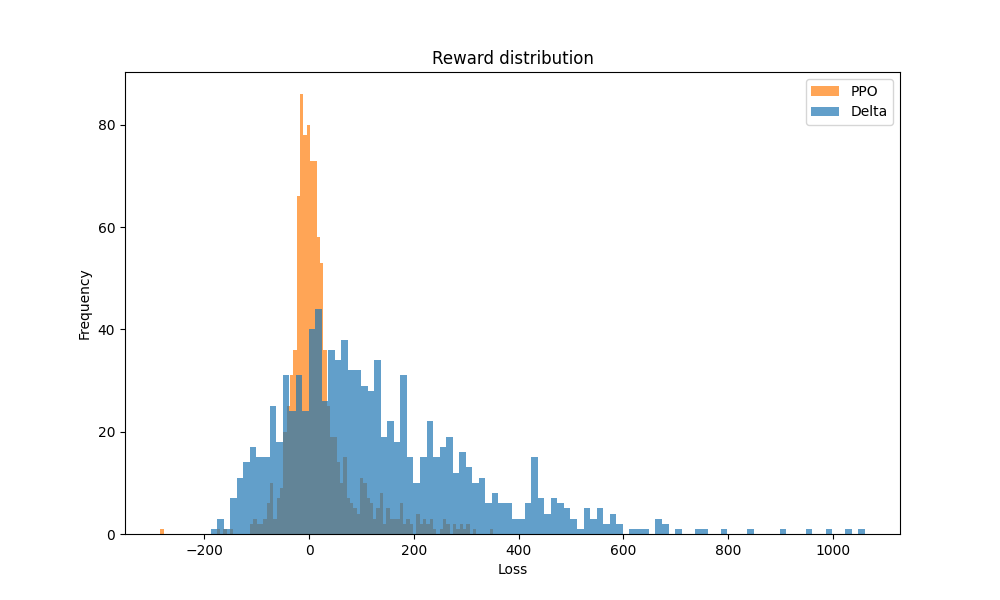
\includegraphics[width=0.8\textwidth]{./project3/figures/reward_distribution.png}
    \caption{Performance of PPO for Hedging GMMB Contracts} 
    \label{fig3:ppo_hedging}
\end{figure}

\section{Transfer Learning for Hedging Variable Annuities}

Transfer learning is a machine learning technique that leverages knowledge gained from one task to improve performance on another related task.
In the context of reinforcement learning, transfer learning can be used to transfer knowledge learned from one environment to another, allowing the agent to learn more efficiently and effectively in the new environment.
In this section, we explore the potential of transfer learning for hedging VAs by transferring knowledge learned from a related financial derivative, such as a European option, to improve the performance of the hedging policy for VAs.

In the context of deep reinforcement learning, transfer learning can be used to improve the risk management of VAs in five ways:
\begin{enumerate}
    \item   \textbf{Transferring to VA products}: Knowledge can be transferred from the hedging strategies of financial derivatives to constructing hedging strategies for VAs.
    VAs are complex insurance products with unique features, which makes it challenging to develop effective hedging strategies.
    However, the payoff structures of VAs are similar to those of financial derivatives, such as European options, which have been extensively studied in the literature.
    By leveraging the knowledge from the hedging strategies of financial derivatives, we can improve the risk management of VAs.
    \item   \textbf{Transferring to new VA products}: Knowledge can be transferred from the hedging strategies of one VA product to another VA product.
    Different VA products have different features and payoff structures, which makes it challenging to develop hedging strategies for new VA products.
    However, experience from hedging one VA product can be transferred to develop hedging strategies for new VA products, especially when the new VA product is similar to the existing ones.
    \item   \textbf{Transferring to new asset models}: Knowledge can be transferred from the hedging strategies of one asset model to another asset model.
    A stochastic volatility model is a more realistic model for asset prices than the Black-Scholes model, but it is more challenging to develop hedging strategies for VAs under such a model.
    \item  \textbf{Transferring to new model specifications}: Model misspecification is a common issue in financial modeling, and training on data simulated with misspecified parameters can lead to suboptimal hedging strategies.
    If only the misspecified model is similar to the correct model, then we can leverage the knowledge from the misspecified model to improve the hedging strategies under the correct model, since the only difference between the two models is the parameter values. 
    \item   \textbf{Transferring to the real world}: Knowledge can be transferred from simulated data to real-world data.
    In practice, it is challenging to obtain real-world data for VAs, but we can leverage simulated data to develop hedging strategies for VAs.
    If the simulated data is representative of the real-world data, then the hedging strategies developed from the simulated data can be transferred to the real world.
\end{enumerate}
Given a set of source domains $\bm{\mathcal{M}}_s= \{ \mathcal{M}_s| \mathcal{M}_s \in \bm{\mathcal{M}}_s\}$ and a target domain $\mathcal{M}_t$, transfer learning aims to improve the learning on the target domain.
While utilizing the interior information $\mathcal{I}_t$ from the target domain, the exterior information $\mathcal{I}_s$ from the source domains is also leveraged to improve the learning on the target domain.
\begin{equation}
    \pi^* = \arg \max_\pi \mathbb{E}_{s \sim \mu_0, a \sim \pi} \left[V_{\mathcal{M}}^\pi (s, a) \right], 
\end{equation}
where $\pi = \phi(\mathcal{I}_s \sim \bm{\mathcal{M}}_s, \mathcal{I}_t \sim \mathcal{M}_t)$ is policy learned from target domain based on information from both the source domains and the target domain.
A regular reinforcement without transfer learning is a special case where $\mathcal{I}_s = \emptyset$ and $\pi = \phi(\mathcal{I}_t \sim \mathcal{M}_t)$.
In the context of deep hedging, various research has been conducted to improve the hedging strategies on real-world data by leveraging knowledge from simulated data.
Most of the research uses the offline-online learning approach, where the hedging strategies are first trained with simulation data, but updated in real-time based on new market information and continuous learning to adapt to changing market dynamics.
The most relevant paper to our study is~\cite{xiao2021optimal}, which use policy gradient algorithms to train hedging strategies for European options with simulation data from Heston model and then updated in real-time hedging S\&P 500 index options.

\subsection{Evaluation Metrics}
The metrics discussed for evaluating transfer learning approaches focus on two key aspects: mastery and generalization. 
Mastery assesses the agent's final performance level in the target domain, indicating how effectively it has learned a specific task from previous knowledge. 
Some common metrics for evaluating mastery include:
\begin{itemize}
    \item \textbf{Asymptotic performance:} the final reward of the agent in the target domain.
    \item \textbf{Transfer ratio:} the ratio of the agent's performance in the target domain with and without transfer learning.
\end{itemize}
Generalization, on the other hand, refers to the agent's ability to quickly adapt its learned knowledge to the target domain.
\begin{itemize}
    \item \textbf{Jumpstart performance:} the initial reward of the agent in the target domain.
    \item \textbf{Accumulated reward:} the total area under the reward curve over time in the target domain.
    \item \textbf{Time to threshold:} the time it takes for the agent to reach a certain performance threshold in the target domain.
    \item \textbf{Performance with fixed epochs:} the agent's performance in the target domain after a fixed number of epochs.
\end{itemize}
